我們需要一種更系統、更嚴格的方式來描述線程通過內存交互、對共享數據的使用,及其對併發應用的影響,這個描述稱為內存模型。內存模型描述了當線程訪問相同的內存位置時存在哪些保證和限制。

C++11標準之前,C++語言沒有內存模型(在標準中沒有提到線程這個詞)。這有什麼問題呢?再來看看我們的生產者-消費者例子(關注生產者方面):

\begin{lstlisting}[style=styleCXX]
std::mutex mN;
size_t N = 0;
…
new (buffer + N) T( … arguments … );
{ // Critical section start – acquire lock
	std::lock_guard l(mN);
	++N;
} // Critical section end - release lock
\end{lstlisting}

\texttt{lock\_guard}只是一個互斥鎖的RAII包裝器,所以不能忘記解鎖:

\begin{lstlisting}[style=styleCXX]
std::mutex mN;
size_t N = 0;
…
new (buffer + N) T( … arguments … ); // N
mN.lock(); // mN
++N; // N
mN.unlock(); // mN
\end{lstlisting}

請注意,這段代碼的每一行都使用了\texttt{N}或\texttt{nM},但從未在一個操作中一起使用。從C++的角度來看,這段代碼可化簡為:

\begin{lstlisting}[style=styleCXX]
size_t n, m;
++m;
++n;
\end{lstlisting}

這段代碼中,操作的順序並不重要,只要可觀察對象的行為沒有改變即可(可觀察對象的行為是輸入和輸出,改變內存中的值不是可觀察對象的行為),編譯器就可以重排它們的順序。回到最初的例子,為什麼編譯器不重新對操作進行排序呢?

\begin{lstlisting}[style=styleCXX]
mN.lock(); // mN
mN.unlock(); // mN
++N; // N
\end{lstlisting}

這將是非常糟糕的,但C++標準(直到C++11)無法阻止編譯器這樣做。

當然,早在2011年之前,我們就已經在用C++編寫多線程程序了,那麼它們是如何工作的呢?顯然,編譯器當時沒有做這樣的優化,原因可以在內存模型中找到。編譯器提供了超出C++標準的某些保證,並提供了特定的內存模型,即使標準不需要這些模型。基於Windows的編譯器遵循Windows內存模型,而大多數基於Unix和Linux的編譯器提供POSIX內存模型和相應的保證。

C++11標準改變了這一點,並賦予了C++內存模型。伴隨原子操作的內存序保證,而鎖是內存模型的一部分。C++內存模型現在保證了跨平臺的可移植性,而以前提供了一組在不同平臺上的保證,每個保證都根據其內存模型進行。此外,C++內存模型提供了一些特定於語言的保證。

我們已經在不同的內存序標準中看到了這些保證:自由、獲取、釋放和獲取-釋放。C++有一個更嚴格的內存順序,稱為\textbf{順序一致}(\texttt{std::memory\_order\_seq\_cst}),這是默認的內存序。不僅每個原子操作都有一個指定順序的雙向內存柵欄,而且整個程序都滿足順序一致性的要求。這個要求表明,程序的行為都按照一個全局順序執行。此外,這個全局順序有一個重要的屬性。在一個處理器上執行的任意兩個操作A和B,使得A在B之前執行。這兩個操作必須以全局順序出現,並且A也在B之前。可以假設一個順序一致的程序,為每個處理器設想有一組牌,每張牌是具體的操作。然後把這些牌放到一起,而不洗牌。一組牌的牌在另一組牌之間進行移動,但同一組牌的順序永遠不會改變,一組卡片就是程序中操作的全局順序。順序一致性是一個理想的屬性,因為它使判斷併發程序的正確性變得更加容易。然而,這往往會以性能為代價。可以用一個非常簡單的基準測試來進行演示,其比較了不同的內存序:

\hspace*{\fill} \\ %插入空行
\noindent
\textbf{05\_barrier\_store.C}
\begin{lstlisting}[style=styleCXX]
void BM_order(benchmark::State& state) {
	for (auto _ : state) {
		x.store(1, memory_order);
		… unroll the loop 32 times for better accuracy …
		x.store(1, memory_order);
		benchmark::ClobberMemory();
	}
	state.SetItemsProcessed(32*state.iterations());
}
\end{lstlisting}

可以使用不同的內存序運行這個基準測試。當然,結果取決於硬件,但下面的結果很罕見:

%\hspace*{\fill} \\ %插入空行
\begin{center}
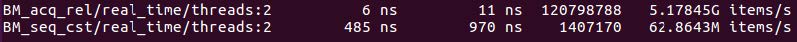
\includegraphics[width=0.9\textwidth]{content/1/chapter5/images/14.jpg}\\
圖5.14 -獲取-釋放與連續一致性內存序的性能
\end{center}

C++內存模型不僅僅是原子操作和內存序。還有,在前面學習偽共享時,假設從多個線程併發地訪問數組相鄰元素是安全的,這些是不同的變量。然而,語言(甚至編譯器)所採用的限制都不能保證。大多數硬件平臺上,訪問整數數組的相鄰元素確實是線程安全的。但對於較小的數據類型(例如\texttt{bool}數組),情況不是這樣。許多處理器使用掩碼整數寫入單個字節,加載包含該字節的整個4字節字,將字節更改為新值,然後將字寫回。顯然,如果兩個處理器同時對共享相同4字節字的兩個字節執行此操作,那麼第二個寫操作將覆蓋第一個寫操作。C++11的內存模型要求,如果沒有兩個線程訪問同一個變量,那麼寫入不同的變量(比如數組元素)都是線程安全的。C++11之前,很容易編寫一個程序來證明從兩個線程寫入兩個相鄰的\texttt{bool}或\texttt{char}變量不是線程安全的。在這本書中沒有這個演示的原因是,今天可用的編譯器不會退回到C++03,即使指定標準級別為C++03(這是不保證的,編譯器可以使用掩碼寫在C++03模式中寫單個字節,大多數編譯器使用與C++11模式相同的指令)。

關於C++內存模型的重要性,最後一個例子也有觀察的價值,語言和編譯器並不都定義了內存模型。硬件有一個內存模型,操作系統和運行時環境有它們的內存模型,程序運行的硬件/軟件系統的每個組件都有一個內存模型。整個內存模型,即程序可用的所有保證和限制的集合,是所有這些內存模型的疊加。有時候,可以利用它,例如:在編寫特定於處理器的代碼時。然而,任何可移植的C++代碼都只能依賴於語言本身的內存模型,並且其他底層內存模型都很複雜。

由於語言的內存模型和硬件的內存模型的不同,出現了兩種問題。首先,程序中可能有一些在特定硬件上無法檢測到的Bug。考慮用於生產者-消費者程序的獲取-釋放協議。如果犯了一個錯誤,在生產者端使用釋放內存序,而在消費者端使用自由內存序(完全沒有柵欄),會期望程序間歇性地產生不正確的結果。但是,如果在x86 CPU上運行這個程序,它似乎是正確的。這是因為x86架構的內存模型是這樣的,每個存儲都伴隨著一個釋放柵欄,而每個加載都有一個隱式的獲取柵欄。當然,程序仍然存在一個漏洞,如果將其移植到基於ARM的處理器(就像iPad上的處理器)上,它就會給我們帶來麻煩。但是在x86硬件上找到這個Bug的唯一方法會用到GCC和Clang中提供的\textbf{Thread santizer(TSAN是一種C/C++數據競爭檢測工具)}工具。

第二個問題與第一個問題相反,減少對內存序的限制並不總是會帶來更好的性能。在一個x86處理器上從釋放到自由內存序寫操作不會帶來任何性能上的提升,因為總的內存模型可以保證釋放順序(理論上,編譯器可能會對自由內存序做更多的優化,而大多數編譯器根本不會優化原子操作)。

內存模型為討論程序如何與內存系統交互提供了科學基礎和通用語言,內存柵欄是開發者在代碼中用來控制內存模型特性的實際工具。通常,這些柵欄是通過使用隱式調用鎖完成的。內存柵欄的最佳使用可以對某些高性能併發程序的效率,產生很大的影響。














